

\section{Environment Domain} \label{sec:env_domain}

\begin{figure*}[t]
    \centering
    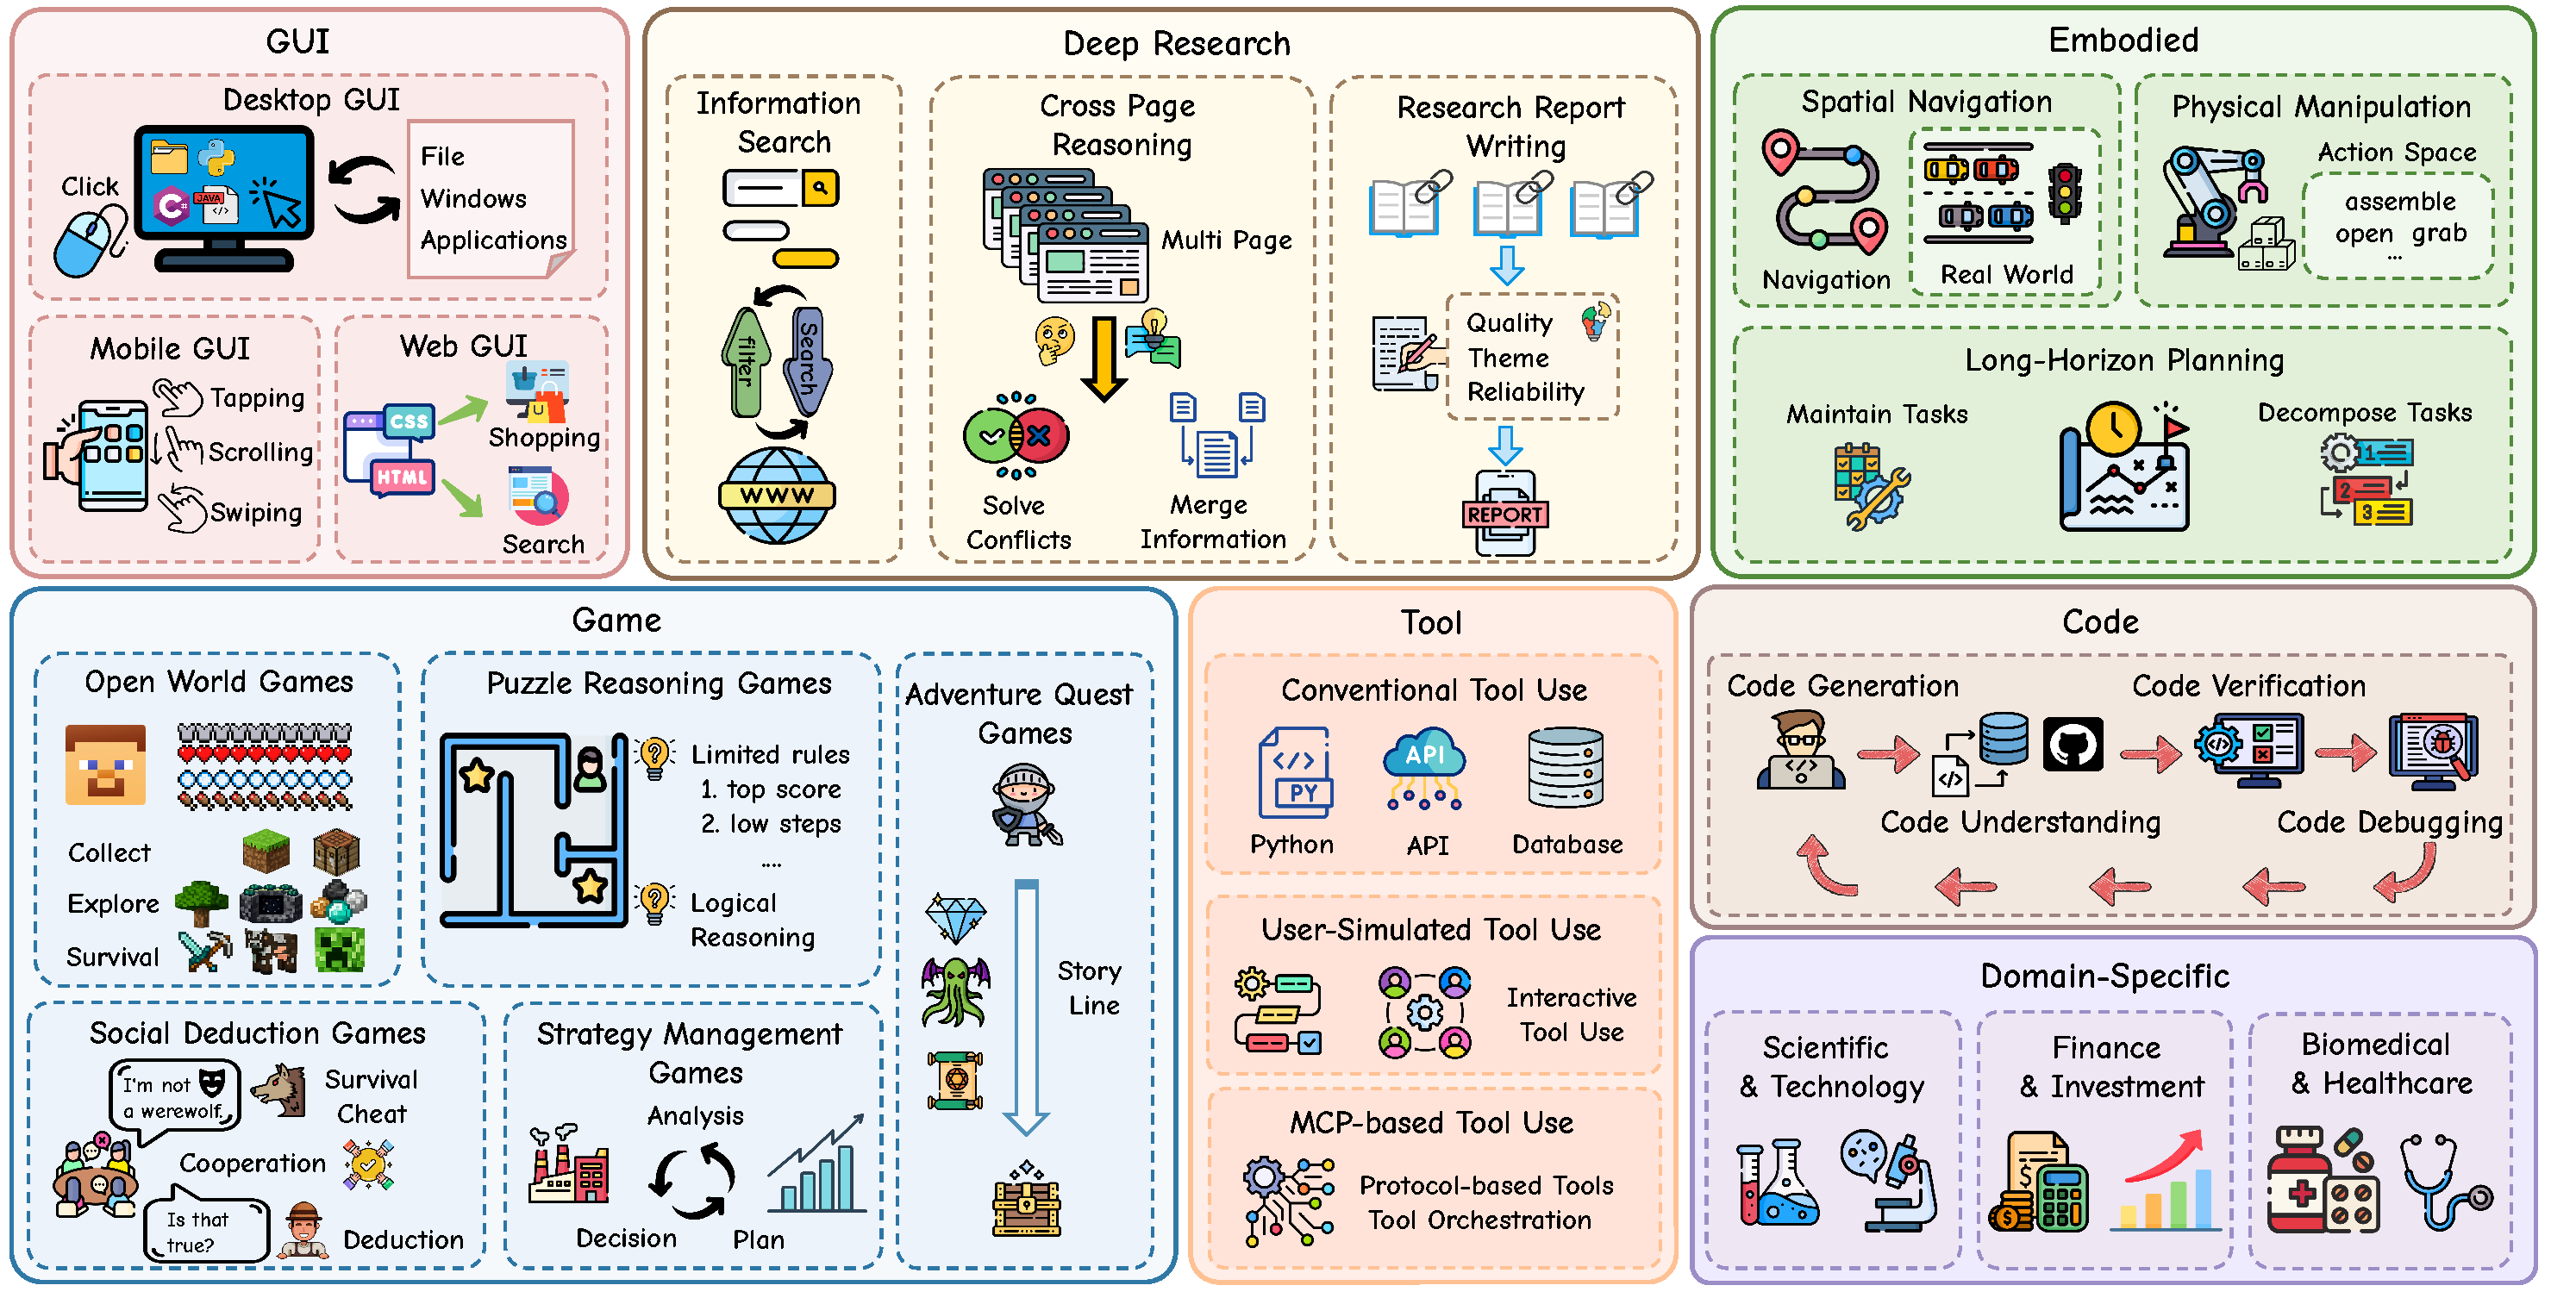
\includegraphics[width=1\textwidth]{images/env_domain.pdf}
    \caption{
    An overview of environment domains, including GUI, Deep Research, Embodied, Game, Tool, Code, and Domain-Specific.
    }
    \label{fig:environment_domain_overview}
\end{figure*}



As shown in Fig. \ref{fig:environment_domain_overview}, agent evaluation spans a diverse set of environments, with different domains placing substantially different demands on agents. Some environments focus on grounded perception and interface manipulation, some emphasize long-horizon planning and interactive decision making, and others require evidence synthesis, tool use, or domain-specific professional reasoning. Consequently, existing evaluation environments can be broadly organized into several domains, including \textbf{GUI} (\cref{GUI}), \textbf{Deep Research} (\cref{sec:Deep Research}), \textbf{Embodied} (\cref{Embodied}), \textbf{Game} (\cref{Game}), \textbf{Tool} (\cref{Tool}), \textbf{Code} (\cref{Code}), \textbf{Domain-Specific} (\cref{Domain-Specific}), and \textbf{Cross-Domain} (\cref{Cross-Domain}). This taxonomy reflects a broader shift in agent evaluation from narrow, task-specific benchmarks toward more diverse, realistic, and capability-compositional environments.


\begin{table*}
\caption{An overview of various environments categorized into \textbf{GUI} and \textbf{Deep Research} domains. Within the Modality column, specific icons are utilized to denote the supported data types where \protect\Text represents text, \protect\Image represents images, and \protect\Video represents videos. Additionally, the \protect\Yes and \protect\No icons indicate the presence or absence of specific attributes across the columns, while the resource icons provide direct links to the respective GitHub \protect\ghlink{https://github.com/} or Hugging Face \protect\hflink{https://huggingface.co/} repositories.}
\resizebox{\textwidth}{!}{
\rowcolors{2}{white}{gray!10} 
\renewcommand{\arraystretch}{1.3}
\begin{tabular}{c|lccccccc} \toprule
\textbf{Domain} & \textbf{Name} & \textbf{Size} & \textbf{Modality} & \textbf{Observability} & \textbf{Multi-agent} & \textbf{Continuity} & \textbf{Online} & \textbf{Resource} \\ \midrule

\cellcolor{white} & WebShop~\cite{WebShop} & 500 & \Text\hspace{-0.4em}\Image & Partially & \No & Discrete & \Yes & \ghlink{https://github.com/princeton-nlp/WebShop}\\
\cellcolor{white} & Mind2Web~\cite{Mind2Web} & 1,341 & \Text\hspace{-0.4em}\Image & Partially & \No & Discrete & \No & \ghlink{https://github.com/OSU-NLP-Group/Mind2Web}\\
\cellcolor{white} & Mind2Web2~\cite{Mind2Web2} & 120 & \Text\hspace{-0.4em}\Image & Partially & \No & Discrete & \Yes & \ghlink{https://github.com/OSU-NLP-Group/Mind2Web-2}\\
\cellcolor{white} & WebArena~\cite{WebArena} & 812 & \Text\hspace{-0.4em}\Image & Partially & \No & Discrete & \Yes & \ghlink{https://github.com/web-arena-x/webarena}\\
\cellcolor{white} & VisualWebArena~\cite{VisualWebArena} & 910 & \Text\hspace{-0.4em}\Image & Partially & \No & Discrete & \Yes & \ghlink{https://github.com/web-arena-x/visualwebarena}\\

\cellcolor{white} & WebVoyager~\cite{WebVoyager} & 643 & \Text\hspace{-0.4em}\Image & Partially & \No & Discrete & \Yes & \ghlink{https://github.com/MinorJerry/WebVoyager}\\
\cellcolor{white} & Mobile-Env~\cite{Mobile-Env} & 74 & \Text\hspace{-0.4em}\Image & Partially & \No & Mixed & \Yes & \ghlink{https://github.com/X-LANCE/Mobile-Env}\\
\cellcolor{white} & AitW~\cite{AitW} & 715,142 & \Text\hspace{-0.4em}\Image & Partially & \No & Mixed & \No & \ghlink{https://github.com/google-research/google-research/tree/master/android_in_the_wild}\\
\cellcolor{white} & AndroidWorld~\cite{AndroidWorld} & 116 & \Text\hspace{-0.4em}\Image & Partially & \No & Mixed & \Yes & \ghlink{https://github.com/google-research/android_world}\\
\cellcolor{white} & AndroidControl~\cite{AndroidControl} & 721 & \Text\hspace{-0.4em}\Image & Partially & \No & Mixed & \No & \ghlink{https://github.com/google-research/google-research/tree/master/android_control}\\

\cellcolor{white} & MobileWorld~\cite{MobileWorld} & 201 & \Text\hspace{-0.4em}\Image & Partially & \No & Mixed & \Yes & \ghlink{https://github.com/Tongyi-MAI/MobileWorld}\\
\cellcolor{white} & AgentStudio~\cite{AgentStudio} & 205 & \Text\hspace{-0.4em}\Image\hspace{-0.4em}\Video & Partially & \No & Mixed & \Yes & \ghlink{https://ltzheng.github.io/agent-studio/}\\
\cellcolor{white} & WorkArena~\cite{WorkArena} & 19,912 & \Text\hspace{-0.4em}\Image & Partially & \No & Mixed & \Yes & \ghlink{https://github.com/ServiceNow/WorkArena}\\
\cellcolor{white} & OSWorld~\cite{OSWorld} & 369 & \Text\hspace{-0.4em}\Image & Partially & \No & Mixed & \Yes & \ghlink{https://github.com/xlang-ai/OSWorld}\\
\cellcolor{white} & WindowsAgentArena~\cite{WindowsAgentArena} & 154 & \Text\hspace{-0.4em}\Image & Partially & \No & Mixed & \Yes & \ghlink{https://github.com/microsoft/WindowsAgentArena}\\

\cellcolor{white} & OSWorld-MCP~\cite{OSWorld-MCP} & 361 & \Text & Partially & \No & Mixed & \Yes & \ghlink{https://github.com/X-PLUG/OSWorld-MCP}\\
\cellcolor{white} & Mobile-Bench~\cite{Mobile-Bench} & 832 & \Text\hspace{-0.4em}\Image 
& Partially & \No & Discrete & \Yes & \ghlink{https://github.com/XiaoMi/MobileBench}\\
\cellcolor{white} & MT-Mind2Web~\cite{MT-Mind2Web} & 120 & \Text & Partially & \No & Discrete & \No & \hflink{https://huggingface.co/datasets/magicgh/MT-Mind2Web}\\
\cellcolor{white} & VideoWebArena~\cite{VideoWebArena} & 2,021 & \Text\hspace{-0.4em}\Image\hspace{-0.4em}\Video & Partially & \No & Mixed & \Yes & \ghlink{https://github.com/ljang0/videowebarena}\\
\cellcolor{white} & Mind2Web-Live~\cite{Mind2Web-Live} & 104 & \Text\hspace{-0.4em}\Image & Partially & \No & Discrete & \Yes & \hflink{https://huggingface.co/datasets/iMeanAI/Mind2Web-Live}\\
\cellcolor{white} & Online-Mind2Web~\cite{Online-Mind2Web} & 300 & \Text\hspace{-0.4em}\Image & Partially & \No & Discrete & \Yes & \hflink{https://huggingface.co/datasets/osunlp/Online-Mind2Web}\\
\cellcolor{white} \multirow{-22}{*}{\makecell{\textbf{GUI} \\ (\cref{GUI})}} & MobileAgentBench~\cite{MobileAgentBench} & 100 & \Text\hspace{-0.4em}\Image & Partially & \No & Mixed & \Yes & \ghlink{https://github.com/MobileAgentBench/mobile-agent-bench}\\
\midrule

\cellcolor{white} & HLE~\cite{HLE} & 2,500 & \Text\hspace{-0.4em}\Image & Partially & \No & Discrete & \Yes & \raisebox{-0.2em}{\hflink{https://huggingface.co/datasets/cais/hle}}\\
\cellcolor{white} & DeepResearch Bench~\cite{DeepResearch-Bench} & 100 & \Text & Partially & \No & Discrete & \Yes & \ghlink{https://github.com/Ayanami0730/deep_research_bench}\\
\cellcolor{white} & GAIA~\cite{GAIA} & 466 & \Text & Partially & \No & Discrete & \Yes & \raisebox{-0.2em}{\hflink{https://huggingface.co/gaia-benchmark}}\\
\cellcolor{white} & WideSearch~\cite{WideSearch} & 200 & \Text & Partially & \No & Discrete & \Yes & \raisebox{-0.2em}{\hflink{https://huggingface.co/datasets/ByteDance-Seed/WideSearch}}\\
\cellcolor{white} & WebWalker~\cite{WebWalker} & 680 & \Text & Partially & \No & Discrete & \Yes & \ghlink{https://github.com/Alibaba-NLP/DeepResearch}\\

\cellcolor{white} & BrowseComp~\cite{BrowseComp} & 1,266 & \Text & Partially & \No & Discrete & \Yes & \ghlink{https://github.com/openai/simple-evals}\\
\cellcolor{white} & Conflicts~\cite{Conflicts} & 458 & \Text & Partially & \No & Discrete & \Yes & \ghlink{https://github.com/google-research-datasets/rag_conflicts}\\
\cellcolor{white} & DeepResearchGym~\cite{DeepResearchGym} & 1,000 & \Text & Partially & \No & Discrete & \Yes & \ghlink{https://github.com/cxcscmu/deepresearch_benchmarking}\\
\cellcolor{white} & InfoDeepSeek~\cite{InfoDeepSeek} & 245 & \Text & Partially & \No & Discrete & \Yes & \ghlink{https://github.com/YunjiaXi/InfoDeepSeek}\\
\cellcolor{white} & InfoSeek~\cite{InfoSeek} & 830 & \Text & Partially & \No & Discrete & \Yes & \ghlink{https://github.com/VectorSpaceLab/Infomatica}\\
\cellcolor{white}   & BrowseComp-ZH~\cite{BrowseComp-ZH} & 289 & \Text & Partially & \No & Discrete & \Yes & \ghlink{https://github.com/PALIN2018/BrowseComp-ZH}\\


\cellcolor{white} & SurveyGen~\cite{SurveyGen} & 4,200 & \Text & Partially & \No & Discrete & \No & \ghlink{https://github.com/tongbao96/SurveyGen}\\
\cellcolor{white} & ReportBench~\cite{ReportBench} & 100 & \Text & Partially & \No & Discrete & \Yes & \ghlink{https://github.com/ByteDance-BandAI/ReportBench}\\
\cellcolor{white} & LiveDRBench~\cite{LiveDRBench} & 100 & \Text & Partially & \No & Discrete & \Yes & \ghlink{https://github.com/microsoft/LiveDRBench}\\
\cellcolor{white} & ScholarQABench~\cite{ScholarQABench} & 2,967 & \Text & Partially & \No & Discrete & \No & \ghlink{https://github.com/AkariAsai/ScholarQABench}\\
\cellcolor{white} & ResearcherBench~\cite{ResearcherBench} & 65 & \Text & Partially & \No & Discrete & \Yes & \ghlink{https://github.com/GAIR-NLP/ResearcherBench}\\
\cellcolor{white} & ProxyQA~\cite{ProxyQA} & 100 & \Text & Partially & \No & Discrete & \No & \ghlink{https://github.com/Namco0816/ProxyQA}\\
\cellcolor{white} & AI Idea Bench 2025~\cite{AI_Idea_Bench_2025} & 3,495 & \Text & Partially & \No & Discrete & \No & \ghlink{https://github.com/yansheng-qiu/AI_Idea_Bench_2025}\\
\cellcolor{white} & DeepReview~\cite{DeepReview} & 13,378 & \Text & Partially & \No & Discrete & \No & \ghlink{https://github.com/ResearAI/DeepReviewer-v2}\\
\cellcolor{white} & PaperBench~\cite{PaperBench} & 20 & \Text & Partially & \No & Discrete & \No & \ghlink{https://github.com/openai/preparedness/tree/main/project/paperbench}\\
\cellcolor{white} & Multimodal-DeepResearcher~\cite{Multimodal_DeepResearcher} & 100 & \Text\hspace{-0.4em}\Image & Partially & \No & Discrete & \Yes & \ghlink{https://github.com/rickyang1114/multimodal-deepresearcher}\\
\cellcolor{white} & Vision-DeepResearch~\cite{Vision_DeepResearch} & 2,000 & \Text\hspace{-0.4em}\Image & Partially & \No & Discrete & \Yes & \ghlink{https://github.com/Osilly/Vision-DeepResearch}\\
\cellcolor{white} & MMDR-Bench~\cite{MMDeepResearch_Bench} & 140 & \Text\hspace{-0.4em}\Image & Partially & \No & Discrete & \Yes & \ghlink{https://github.com/AIoT-MLSys-Lab/MMDeepResearch-Bench}\\
\cellcolor{white} \multirow{-25}{*}{\makecell{\textbf{Deep Research} \\ (\cref{sec:Deep Research})}} & OmniGAIA~\cite{OmniGAIA} & 360 & \Text\hspace{-0.4em}\Image\hspace{-0.4em}\Video & Partially & \No & Discrete & \Yes & \ghlink{https://github.com/RUC-NLPIR/OmniGAIA}\\

 \bottomrule
\end{tabular}}
\end{table*}



\subsection{GUI}
\label{GUI}
\textbf{GUI} environments denote settings in which agents complete tasks through the perception and manipulation of graphical user interfaces~\cite{OSWorld,WindowsAgentArena,AgentStudio,AitW,Mobile-Env,AndroidWorld,MobileAgentBench,WebShop,Mind2Web,WebArena,VisualWebArena}. These environments emphasize the ability to comprehend, localize and interact with interface elements, as well as to make sequential decisions and execute actions based on interface feedback. Based on the primary interaction platforms, existing work can be broadly categorized into three groups: \textbf{Desktop GUI} (\cref{Desktop GUI}), \textbf{Mobile GUI} (\cref{Mobile GUI}), and \textbf{Web GUI} (\cref{Web GUI}).

\subsubsection{Desktop GUI}
\label{Desktop GUI}
\textbf{Desktop GUI} concerns tasks carried out in operating systems, where agents need to interact with files, windows, applications, and system tools. Compared with other GUI settings, this domain places greater demands on long-horizon planning, cross application coordination, and stable grounding in complex visual interfaces. OSWorld~\cite{OSWorld} evaluates open-ended tasks in realistic desktop environments and covers a wide range of everyday computer operations. WindowsAgentArena~\cite{WindowsAgentArena} further focuses on practical Windows workflows and highlights the challenges of interacting with native system components and desktop software. AgentStudio~\cite{AgentStudio} complements these environments by providing a more general platform for building and evaluating GUI agents, which supports broader research on desktop interaction. Overall, Desktop GUI is moving toward more realistic and more general computer use, making it an important domain for evaluating general purpose agents.

\subsubsection{Mobile GUI}
\label{Mobile  GUI}
\textbf{Mobile GUI} focuses on agent interaction with smartphone interfaces, where tasks are completed through tapping, typing, scrolling, and swiping on small screens. Compared with desktop settings, mobile environments are more constrained by limited display space, deeper page transitions, and stronger dependence on app specific layouts. AitW~\cite{AitW} studies Android control from human demonstrations and natural language instructions, establishing mobile GUI as an important grounded interaction problem. Mobile-Env~\cite{Mobile-Env} moves this line of research toward controllable evaluation by providing an interactive Android environment for task construction and testing. More recent benchmarks such as AndroidWorld~\cite{AndroidWorld} and MobileAgentBench~\cite{MobileAgentBench} further emphasize executable and reproducible evaluation, pushing the field from static demonstration data toward realistic mobile task completion. Overall, Mobile GUI has gradually evolved from static demonstration-based settings toward more interactive and realistic mobile environments, making it a key domain for evaluating end-to-end mobile agents.

\subsubsection{Web GUI}
\label{Web GUI}
\textbf{Web GUI} centers on agent interaction with browser interfaces to perform tasks such as navigation, information retrieval, form filling, and shopping. Compared with other GUI settings, this domain combines textual content, visual layout, structured page elements, and dynamic interaction logic, which makes it one of the main testbeds for GUI agents. WebShop~\cite{WebShop} frames online shopping as sequential decision making over webpages. Mind2Web~\cite{Mind2Web} extends this setting to real websites from diverse domains and highlights generalization to unseen sites and tasks. WebArena~\cite{WebArena} further advances the field by providing executable web environments for realistic long-horizon workflows, while VisualWebArena~\cite{VisualWebArena} shows that rendered visual information is often necessary for successful web interaction. Web GUI now serves as a central benchmark for studying agent performance in dynamic, information-rich, and workflow-oriented online environments.

\subsection{Deep Research}
\label{sec:Deep Research}
% Deep Research 是指智能体围绕开放式研究目标，在网页、搜索引擎、数据库和文档库中持续进行信息检索、证据筛选、来源核验与结果整合，最终形成有依据的回答或研究报告。与只要求单步检索或单页问答的任务不同，Deep Research 更强调长程信息搜集、跨来源证据整合以及面向用户目标的结果组织能力。按照任务链路中的主要瓶颈，现有工作大致可以分为 \textbf{Information Search}、\textbf{Cross Page Reasoning} 和 \textbf{Research Report Writing} 三类。前一类关注能否找到信息，中间一类关注能否整合信息，后一类关注能否产出结构化研究结果。

\textbf{Deep Research} refers to the process where an agent continuously retrieves information, screens evidence, and synthesizes findings from diverse sources to address a research goal, ultimately generating answers grounded in evidence. Based on the major bottlenecks involved, existing work can be broadly divided into three categories (\cref{Information Search,Multi-Source Reasoning,Research Report Writing}). The first~\cite{WebWalker,WideSearch,InfoDeepSeek} centers on finding relevant information, referred to as \textbf{Information Search}; the second~\cite{GAIA,BrowseComp,Conflicts,BrowseComp-ZH} emphasizes synthesizing information across sources, referred to as \textbf{Multi-Source Reasoning}; and the third~\cite{DeepResearch-Bench,DeepResearchGym,DR_BENCH} targets the production of structured research outputs, referred to as \textbf{Research Report Writing}.


\subsubsection{Information Search}
\label{Information Search}
\textbf{Information Search} examines whether an agent can effectively search the open web and progressively extend its exploration to uncover high quality evidence. SimpleQA~\cite{SimpleQA} evaluates the ability to retrieve precise factual information for question answering, capturing the most basic form of web information seeking. 
WideSearch~\cite{WideSearch} focuses on broad information collection across sources, highlighting the gathering and organization of large numbers of atomic facts. 
InfoDeepSeek~\cite{InfoDeepSeek} evaluates information gathering in Agentic RAG as a standalone capability, focusing on how agents decide whether to search, what to search for, and which evidence to retain.
Overall, this line of work shifts Deep Research from single retrieval to persistent exploration and from finding a single answer to covering a body of valuable evidence.


\subsubsection{Multi-Source Reasoning}
\label{Multi-Source Reasoning}
\textbf{Multi-Source Reasoning} concerns whether an agent can synthesize information from multiple sources by comparing evidence, aligning claims, drawing inferences, and resolving conflicts. GAIA~\cite{GAIA} requires models to combine reasoning, web browsing, and tool use to solve real world problems that often cannot be answered from a single page. 
WebWalker~\cite{WebWalker} also relates to this setting, as solving its tasks often requires agents to move through hierarchical website structures and connect evidence distributed across multiple linked pages. 
BrowseComp~\cite{BrowseComp} further highlights this ability by requiring sustained navigation and the integration of scattered clues, making it well suited for evaluating cross page evidence synthesis. 
Conflicts~\cite{Conflicts} focuses explicitly on contradictions across sources, testing whether models can detect conflicts and distinguish their types. With benchmarks such as BrowseComp-ZH~\cite{BrowseComp-ZH}, this line of work has also expanded from English webpages to more complex Chinese information environments. Overall, the key capability in Deep Research is not reproducing a single source but relating multiple pieces of evidence to form a grounded conclusion.


\subsubsection{Research Report Writing}
\label{Research Report Writing}
\textbf{Research Report Writing} concerns whether an agent can transform collected evidence into structured, verifiable research outputs that are aligned with user needs. DeepResearch Bench~\cite{DeepResearch-Bench} evaluates deep research agents with an emphasis on iterative web exploration, targeted retrieval, advanced synthesis, and report quality. DeepResearchGym~\cite{DeepResearchGym} highlights reproducible evaluation by providing stable search interfaces and protocols for more controlled comparison of report generation. DR.BENCH~\cite{DR_BENCH} focuses more directly on long research reports, using a multidimensional framework that evaluates not only content quality but also topical focus and retrieval reliability. Overall, while earlier work mainly evaluates key stages of the research process, such as information search and multi-source reasoning, this line of work shifts the focus toward the quality of the final deliverable.



\begin{table*}
\caption{An overview of various environments categorized into \textbf{Embodied} and \textbf{Game} domains.}
\resizebox{\textwidth}{!}{
\rowcolors{2}{white}{gray!10} 
\renewcommand{\arraystretch}{1.3}
\begin{tabular}{c|lccccccc} 
\toprule
\textbf{Domain} & \textbf{Name} & \textbf{Size}  & \textbf{Modality} & \textbf{Observability} & \textbf{Multi-agent} & \textbf{Continuity} & \textbf{Online} & \textbf{Resource} \\ \midrule
\cellcolor{white} & Habitat~\cite{Habitat} & -- & \Image & Partially & \No & Discrete & \Yes & \ghlink{https://github.com/peteanderson80/Matterport3DSimulator}\\
\cellcolor{white} & Room-to-Room~\cite{Room-to-Room} & 4173 & \Text\hspace{-0.4em}\Image & Partially & \No & Discrete & \Yes & \ghlink{https://github.com/peteanderson80/Matterport3DSimulator}\\
\cellcolor{white} & RLBench~\cite{RLBench} & 100 & \Text\hspace{-0.4em}\Image & Partially & \No & Mixed & \Yes & \ghlink{https://github.com/stepjam/RLBench}\\
\cellcolor{white} & ALFRED~\cite{ALFRED} & 1,529 & \Text\hspace{-0.4em}\Image & Partially & \No & Discrete & \No & \ghlink{https://github.com/askforalfred/alfred}\\
\cellcolor{white} & ALFWorld~\cite{ALFWorld} & 134 & \Text & Partially & \No & Discrete & \Yes & \ghlink{https://github.com/alfworld/alfworld}\\
\cellcolor{white} & Robocasa~\cite{Robocasa} & 100 & \Image & Partially & \No & Continuous & \Yes & \ghlink{https://github.com/robocasa/robocasa}\\
\cellcolor{white} & BEHAVIOR~\cite{BEHAVIOR} & 100 & \Image & Partially & \No & Continuous & \Yes & \ghlink{https://stanfordvl.github.io/behavior/intro.html}\\
\cellcolor{white} & panda-gym~\cite{panda-gym} & 80 & \Text & Completely & \No & Continuous & \Yes & \ghlink{https://github.com/qgallouedec/panda-gym}\\
\cellcolor{white} & MetaDrive~\cite{MetaDrive} & 100 & \Image & Partially & \Yes & Continuous & \Yes & \ghlink{https://github.com/metadriverse/metadrive}\\
\cellcolor{white} & ScienceWorld~\cite{ScienceWorld} & 1,800 & \Text & Partially & \No & Discrete & \Yes & \ghlink{https://github.com/allenai/ScienceWorld}\\
\cellcolor{white} & ET-Plan-Bench~\cite{ET-Plan-Bench} & 11,838 & \Text\hspace{-0.4em}\Image & Partially & \No & Discrete & \Yes & \ghlink{https://github.com/ET-Plan-Bench/ET-Plan-Bench}\\
\cellcolor{white} & LEGENT~\cite{LEGENT} & 100 & \Text\hspace{-0.4em}\Image & Partially & \No & Mixed & \Yes & \ghlink{https://github.com/thunlp/LEGENT}\\
\cellcolor{white} & EmbodiedBench~\cite{EmbodiedBench} & 1,128 & \Text\hspace{-0.4em}\Image & Partially & \No & Mixed & \Yes & \ghlink{https://github.com/EmbodiedBench/EmbodiedBench}\\
\cellcolor{white} & RoboFactory~\cite{RoboFactory} & 1,100 & \Image & Partially & \Yes & Continuous & \Yes & \ghlink{https://github.com/MARS-EAI/RoboFactory}\\
\cellcolor{white} & Scenario Dreamer~\cite{Scenario_Dreamer} & 50,000 & \Image & Partially & \No & Continuous & \Yes & \ghlink{https://github.com/princeton-computational-imaging/scenario-dreamer}\\
\cellcolor{white} & SimuHome~\cite{SimuHome} & 600 & \Text & Partially & \No & Discrete & \Yes & \ghlink{https://github.com/holi-lab/SimuHome}\\
\cellcolor{white} & Sari Sandbox~\cite{Sari_Sandbox} & 100 & \Text\hspace{-0.4em}\Image & Partially & \No & Mixed & \Yes & \ghlink{https://github.com/upeee/sari-sandbox-env}\\
\cellcolor{white} \multirow{-18}{*}{\makecell{\textbf{Embodied}\\(\cref{Embodied}) }} & Nexus~\cite{Nexus} & 1,090 & \Image & Completely & \Yes & Continuous & \No & \ghlink{https://github.com/OpenDriveLab/Nexus}\\ 
\midrule

\cellcolor{white} & MineDojo~\cite{MineDojo} & 3,142 & \Text\hspace{-0.4em}\Image & Partially & \No & Discrete & \Yes & \ghlink{https://github.com/MineDojo/MineDojo}\\
\cellcolor{white} & KORGym~\cite{KORGym} & 55,200 & \Text\hspace{-0.4em}\Image & Partially & \No & Discrete & \Yes & \ghlink{https://github.com/multimodal-art-projection/KORGym}\\
\cellcolor{white} & TextArena~\cite{TextArena} & 74 & \Text & Partially & \Yes & Discrete & \Yes & \ghlink{https://github.com/TextArena/TextArena}\\
\cellcolor{white} & V-GameGym~\cite{V-GameGym} & 2,219 & \Text & Completely & \No & Discrete & \No & \raisebox{-0.2em}{\hflink{https://huggingface.co/datasets/alibabagroup/SKYLENAGE-GameCodeGym}}\\
\cellcolor{white} & Kor-Bench~\cite{KOR-Bench} & 1,250 & \Text & Completely & \No & Discrete & \No & \ghlink{https://github.com/KOR-Bench/KOR-Bench}\\
\cellcolor{white} & AI Gamestore~\cite{AI_GAMESTORE} & 2,100 & \Image & Partially & \No & Mixed & \Yes & \ghlink{https://github.com/lance-ying/aigamestore_harness}\\
\cellcolor{white} & ING-VP~\cite{ING-VP} & 300 & \Image & Partially & \No & Discrete & \Yes & \ghlink{https://github.com/thisisus7/ing-vp}\\
\cellcolor{white} & VideoGameBench~\cite{VideoGameBench} & 50 & \Image & Partially & \No & Mixed & \Yes & \ghlink{https://github.com/alexzhang13/videogamebench}\\
\cellcolor{white} & GVGAI-LLM~\cite{GVGAI-LLM} & 540 & \Text & Completely & \No & Discrete & \Yes & \ghlink{https://github.com/zmuhls/gvgai-web}\\
\cellcolor{white} & BALROG~\cite{BALROG} & 425 & \Text\hspace{-0.4em}\Image & Partially & \No & Discrete & \Yes & \ghlink{https://github.com/balrog-ai/BALROG}\\
\cellcolor{white} & Smartplay~\cite{SMARTPLAY} & 931,900 & \Text & Partially & \No & Discrete & \Yes & \ghlink{https://github.com/microsoft/SmartPlay}\\
\cellcolor{white} & DSGBench~\cite{DSGBench} & 160 & \Image & Partially & \Yes & Discrete & \Yes & \ghlink{https://github.com/DeciBrain-Group/DSGBench}\\
\cellcolor{white} & GTBench~\cite{GTBENCH} & 500 & \Text & Partially & \Yes & Discrete & \Yes & \ghlink{https://github.com/jinhaoduan/GTBench}\\
%\cellcolor{white} & Lmage-Bench~\cite{LMGAME-BENCH} & 319 & \Image & Partially & \No & Discrete & \Yes & \ghlink{https://github.com/lmgame-org/GamingAgent}\\
%\cellcolor{white} & Factorio Learning Environment~\cite{FactorioLearningEnvironment} & 96 & \Text & Partially & \No & Discrete & \Yes & \ghlink{https://github.com/JackHopkins/factorio-learning-environment}\\
\cellcolor{white} & Pok\'eLLMon~\cite{PokeLLMon} & 1,909 & \Text & Partially & \Yes & Discrete & \Yes & \ghlink{https://github.com/git-disl/PokeLLMon}\\
\cellcolor{white} & MC-Planner~\cite{MC-Planner} & 2,130 & \Text\hspace{-0.4em}\Image & Partially & \No & Mixed & \Yes & \ghlink{https://github.com/CraftJarvis/MC-Planner}\\
\cellcolor{white} & GameTraversalBenchmark~\cite{GameTraversalBenchmark} & 150 & \Text & Completely & \No & Discrete & \Yes & \ghlink{https://github.com/umair-nasir14/Game-Traversal-Benchmark}\\
%\cellcolor{white} & FlashAdventure~\cite{FlashAdventure} & 238 & \Image & Partially & \No & Mixed & \Yes & \ghlink{https://github.com/ahnjaewoo/FlashAdventure}\\
\cellcolor{white} & LMRL Gym~\cite{LMRLGym} & 6,541 & \Text & Partially & \No & Discrete & \Yes & \ghlink{https://github.com/abdulhaim/LMRL-Gym}\\
%\cellcolor{white} & MAgIC~\cite{MAgIC} & 375 & \Text & Partially & \Yes & Discrete & \Yes & \ghlink{https://github.com/cathyxl/MAgIC}\\
\cellcolor{white} & Clembench~\cite{clembench} & 250 & \Text & Partially & \Yes & Discrete & \Yes & \ghlink{https://github.com/clp-research/clembench}\\
\cellcolor{white} & Baba Is AI~\cite{BabaIsAI} & 1,275 & \Image & Completely & \No & Discrete & \Yes & \ghlink{https://github.com/nacloos/baba-is-ai}\\
\cellcolor{white} & HLA~\cite{HLA} & 330 & \Text\hspace{-0.4em}\Image & Completely & \Yes & Discrete & \Yes & \ghlink{https://github.com/HosnLS/Hierarchical-Language-Agent}\\
\cellcolor{white} & LLMArena~\cite{LLMARENA} & 5,600 & \Text & Partially & \Yes & Discrete & \Yes & \ghlink{https://github.com/THU-BPM/LLMArena}\\
%\cellcolor{white} & WhodunitBench~\cite{WhodunitBench} & 3,050 & \Text\hspace{-0.4em}\Image & Partially & \No & Discrete & \Yes & \ghlink{https://github.com/jun0wanan/WhodunitBench-Murder_Mystery_Games}\\
\cellcolor{white} & TextGames~\cite{TEXTGAMES} & 24,000 & \Text & Completely & \No & Discrete & \Yes & \ghlink{https://github.com/fhudi/textgames}\\
\cellcolor{white} & GameArena~\cite{GameArena} & 2,240 & \Text & Partially & \Yes & Discrete & \Yes & \ghlink{https://github.com/lmgame-org/ai-space-escape-engine}\\
\cellcolor{white} & SPIN-Bench~\cite{SPIN-Bench} & 1,280 & \Text & Partially & \Yes & Discrete & \Yes & \ghlink{https://github.com/spinbench/spinbench}\\
\cellcolor{white} & GAMEBoT~\cite{GAMEBoT} & 2,720 & \Text & Partially & \Yes & Discrete & \Yes & \ghlink{https://github.com/Visual-AI/GAMEBoT}\\
\cellcolor{white} & GameBench~\cite{GAMEBENCH} & 277 & \Text & Partially & \Yes & Discrete & \Yes & \ghlink{https://github.com/Joshuaclymer/GameBench}\\
\cellcolor{white} & MineWorld~\cite{MINEWORLD} & 1,000 & \Image & Partially & \No & Mixed & \Yes & \ghlink{https://github.com/microsoft/mineworld}\\
\cellcolor{white} & AvalonBench~\cite{AvalonBench} & 1,140 & \Text & Partially & \Yes & Discrete & \Yes & \ghlink{https://github.com/jonathanmli/Avalon-LLM}\\
\cellcolor{white} & Werewolf~\cite{Werewolf} & 1,200 & \Text & Partially & \Yes & Discrete & \Yes & \ghlink{https://github.com/boluoweifenda/werewolf}\\
%\cellcolor{white} & gg-bench~\cite{gg-bench} & 3,780 & \Text & Completely & \Yes & Discrete & \Yes & \ghlink{https://github.com/vivek3141/gg-bench}\\
\cellcolor{white} & GameFactory~\cite{GAMEFACTORY} & 7,407 & \Image\hspace{-0.4em}\Video & Partially & \No & Mixed & \No & \ghlink{https://github.com/KlingAIResearch/GameFactory}\\
\cellcolor{white} & GameNGen~\cite{GameNGen} & 8,912 & \Image\hspace{-0.4em}\Video & Partially & \No & Mixed & \Yes & \ghlink{https://github.com/GameNGen/GameNGen.github.io}\\
%\cellcolor{white} & DeepPHY~\cite{DeepPHY} & 1,336 & \Image & Partially & \No & Discrete & \Yes & \ghlink{https://github.com/ADAPT-Chase/deepphy}\\
%\cellcolor{white} & GameDevBench~\cite{GameDevBench} & 132 & \Text\hspace{-0.4em}\Image\hspace{-0.4em}\Video & Partially & \No & Discrete & \Yes & \ghlink{https://github.com/waynchi/gamedevbench}\\
%\cellcolor{white} & CivRealm~\cite{CivRealm} & 100,000 & \Text & Partially & \Yes & Discrete & \Yes & \ghlink{https://github.com/bigai-ai/civrealm}\\
% \cellcolor{white}  & Novel Games~\cite{NovelGames} & -- & \Text\hspace{-0.4em}\Image & Partially & \No & Discrete & \Yes & --\\ 

\cellcolor{white} & OGC~\cite{OGC} & 37 & \Image & Partially & \Yes & Discrete & \Yes & \ghlink{https://git.hcics.simtech.uni-stuttgart.de/public-projects/OGC}\\
%\cellcolor{white} & Collab-Overcooked~\cite{Collab_Overcooked} & 30 & \Text & Partially & \Yes & Discrete & \Yes & \ghlink{https://github.com/YusaeMeow/Collab-Overcooked}\\
% \cellcolor{white} &ReCon~\cite{ReCon} & 6 & \Text & Partially & \Yes & Discrete & \Yes & \ghlink{https://github.com/shenzhi-wang/avalon_recon}\\
\cellcolor{white} \multirow{-27}{*}{\makecell{\textbf{Game} \\ (\cref{Game})}} & Minigrid \& Miniworld~\cite{Minigrid_Miniworld} & 35 & \Text\hspace{-0.4em}\Image & Partially & \No & Discrete & \Yes & \ghlink{https://github.com/Farama-Foundation/Minigrid}\\

\bottomrule
\end{tabular}}
\end{table*}


\subsection{Embodied}
\label{Embodied}
\textbf{Embodied} environments refer to settings in which an agent acts as a robot or virtual character situated in a 3D environment. In these settings, the agent completes tasks through perception, movement, and interaction~\cite{Habitat,Room-to-Room,MetaDrive,RLBench,Robocasa,BEHAVIOR,ALFRED,ALFWorld,TEAch,ReALFRED}. According to the primary task forms and capability requirements, existing work can be broadly categorized into three types: \textbf{Spatial Navigation} (\cref{Spatial Navigation}), \textbf{Physical Manipulation} (\cref{Physical Manipulation}), and \textbf{Long-Horizon Planning} (\cref{Long-Horizon Planning}).

\subsubsection{Spatial Navigation}
\label{Spatial Navigation}
\textbf{Spatial Navigation} environments center on tasks that require agents to move, explore, localize, and reach target positions in 3D spaces. This line of research mainly examines whether an agent can build usable spatial representations from egocentric observations and act reliably in unseen environments. 
Habitat~\cite{Habitat} provides efficient photorealistic 3D simulation and supports standard embodied tasks such as point goal navigation. Room-to-Room~\cite{Room-to-Room} further extends this setting to language guided navigation in real building scale environments, highlighting the need to ground natural language instructions in perception and action. MetaDrive~\cite{MetaDrive} broadens navigation oriented embodied evaluation to driving scenarios by generating diverse road environments and testing generalization under dynamic traffic conditions. Spatial navigation has become a core setting for evaluating spatial perception and generalization in embodied agents.

\subsubsection{Physical Manipulation}
\label{Physical Manipulation}
\textbf{Physical Manipulation} environments focus on embodied interaction between agents and objects, including tasks such as grasping, placing, assembling and tool use. Compared with navigation tasks, this setting places greater emphasis on precise control, complex contact-rich interaction, and reasoning about object states. RLBench~\cite{RLBench} provides a large scale manipulation benchmark with diverse vision-guided tasks and supports research on multi-task and imitation-based robot learning. Robocasa~\cite{Robocasa} extends this direction toward realistic everyday household tasks and language-conditioned mobile manipulation. BEHAVIOR~\cite{BEHAVIOR} further improves realism by modeling a wide range of everyday household activities, while also showing that current embodied agents still exhibit clear limitations in complex physical interaction. Physical manipulation has expanded from narrow skill evaluation to more general and realistic object-centric interaction settings.

\subsubsection{Long-Horizon Planning}
\label{Long-Horizon Planning}
\textbf{Long-Horizon Planning} environments center on multi step and compositional tasks whose success depends on maintaining task state, decomposing goals, and adapting to changing environments. In this setting, the main challenge is not only to execute individual actions, but also to organize them into coherent plans over long decision horizons.
ALFRED~\cite{ALFRED} is a representative benchmark in this area, as it combines egocentric vision and natural language instructions with long household tasks that involve irreversible state changes. ALFWorld~\cite{ALFWorld} complements this direction by aligning text based and embodied environments, making it possible to study abstract planning together with grounded execution. TEACh~\cite{TEAch} further extends long-horizon embodied tasks to dialogue-enabled settings, where agents must complete household goals through both interaction and clarification. ReALFRED~\cite{ReALFRED} pushes this line toward more realistic environments by reducing the visual and scene gap between simulation and real-world deployment. Long-horizon planning has become an important setting for evaluating planning consistency and long-term task execution in embodied agents.

\begin{table*}[tbp]
\caption{An overview of various environments categorized into \textbf{Tool} and \textbf{Code} domains.}
\resizebox{\textwidth}{!}{
\rowcolors{2}{white}{gray!10} 
\renewcommand{\arraystretch}{1.3}
\begin{tabular}{c|lccccccc} \toprule
\textbf{Domain} & \textbf{Name} & \textbf{Size}  & \textbf{Modality} & \textbf{Observability} & \textbf{Multi-agent} & \textbf{Continuity} & \textbf{Online} & \textbf{Resource} \\ \midrule

\cellcolor{white} & API-Bank~\cite{API-Bank} & 314 & \Text & Completely & \No & Mixed & \Yes & \ghlink{https://github.com/AlibabaResearch/DAMO-ConvAI/tree/main/api-bank}\\
\cellcolor{white} & ToolBench~\cite{ToolBench} & 600 & \Text & Completely & \No & Mixed & \Yes & \ghlink{https://github.com/OpenBMB/ToolBench}\\
\cellcolor{white} & ToolEyes~\cite{ToolEyes} & 382 & \Text & Partially & \No & Discrete & \Yes & \ghlink{https://github.com/Junjie-Ye/ToolEyes}\\
\cellcolor{white} & AppWorld~\cite{AppWorld2024} & 585 & \Text & Partially & \No & Discrete & \Yes & \ghlink{https://github.com/stonybrooknlp/appworld}\\
\cellcolor{white} & $\tau$-bench~\cite{tau-bench} & 165 & \Text & Partially & \No & Mixed & \Yes & \ghlink{https://github.com/sierra-research/tau-bench}\\
\cellcolor{white} & ACEBench~\cite{ACEBench} & 2,000 & \Text & Partially & \No & Discrete & \Yes & \ghlink{https://github.com/chenchen0103/ACEBench}\\
\cellcolor{white} & FlowBench~\cite{FlowBench} & 536 & \Text & Partially & \No & Discrete & \Yes & \ghlink{https://github.com/Justherozen/FlowBench}\\
\cellcolor{white} & TRAJECT-Bench~\cite{TRAJECT-Bench} & 200 & \Text & Partially & \No & Discrete & \No & \hflink{https://huggingface.co/datasets/bigboss24/TRAJECT-Bench}\\
\cellcolor{white} & ETAPP~\cite{ETAPP} & 800 & \Text & Partially & \No & Mixed & \Yes & \ghlink{https://github.com/hypasd-art/ETAPP}\\
\cellcolor{white} & BFCL~\cite{BFCL} & 5,551 & \Text & Partially & \No & Discrete & \Yes & \ghlink{https://github.com/ShishirPatil/gorilla/tree/main}\\
\cellcolor{white} & UserBench~\cite{UserBench} & 471 & \Text & Partially & \No & Discrete & \Yes & 
\ghlink{https://github.com/SalesforceAIResearch/UserBench/tree/main}\\
\cellcolor{white} & $\tau$2-bench~\cite{tau2-bench} & 279 & \Text & Partially & \Yes & Discrete & \Yes & \ghlink{https://github.com/sierra-research/tau2-bench}\\
\cellcolor{white} & MCPVerse~\cite{MCPVerse} & 250 & \Text & Partially & \No & Mixed & \Yes & \ghlink{https://github.com/hailsham/mcpverse}\\
\cellcolor{white} & MCPToolBench++~\cite{MCPToolBench++} & 1,509 & \Text & Partially & \No & Discrete & \Yes & \ghlink{https://github.com/mcp-tool-bench/MCPToolBenchPP}\\
\cellcolor{white} & MCP-Universe~\cite{MCP-Universe} & 231 & \Text & Partially & \No & Mixed & \Yes & \hflink{https://huggingface.co/datasets/AfterQuery/MCP-Universe}\\
\cellcolor{white} & MCP-Bench~\cite{MCP-Bench} & 104 & \Text & Partially & \No & Discrete & \Yes & \ghlink{https://github.com/Accenture/mcp-bench}\\
\cellcolor{white} & MCPMark~\cite{MCPMark} & 127 & \Text & Partially & \No & Mixed & \Yes & \ghlink{https://github.com/eval-sys/mcpmark}\\
\cellcolor{white} \multirow{-18}{*}{\makecell{\textbf{Tool} \\ (\cref{Tool})}} & M$^3$-Bench~\cite{M^3-Bench}
& 208 & \Text\hspace{-0.4em}\Image & Partially & \No & Discrete & \Yes & \ghlink{https://github.com/EtaYang10th/Open-M3-Bench}\\

\midrule

\cellcolor{white} & SWE-Bench~\cite{SWE-Bench} & 2,294 & \Text & Partially & \No & Discrete & \Yes & \raisebox{-0.2em}{\hflink{https://huggingface.co/datasets/SWE-bench/SWE-bench}}\\
\cellcolor{white} & InterCode~\cite{InterCode} & 1,351 & \Text & Partially & \No & Discrete & \Yes & \ghlink{https://github.com/princeton-nlp/intercode}\\
\cellcolor{white} & CodeAgent~\cite{CodeAgent} & 101 & \Text & Partially & \No & Discrete & \Yes & \ghlink{https://github.com/zkcpku/CodeAgent}\\
\cellcolor{white} & BigCodeBench~\cite{BigCodeBench} & 1,140 & \Text & Completely & \No & Discrete & \Yes & \raisebox{-0.2em}{\hflink{https://huggingface.co/datasets/bigcode/bigcodebench}}\\
\cellcolor{white} & CodeElo~\cite{CODEELO} & 387 & \Text & Completely & \No & Discrete & \Yes & \raisebox{-0.2em}{\hflink{https://huggingface.co/datasets/Qwen/CodeElo}}\\
\cellcolor{white} & LiveCodeBench~\cite{LiveCodeBench} & 511 & \Text & Completely & \No & Discrete & \Yes & \raisebox{-0.2em}{\hflink{https://huggingface.co/datasets/livecodebench/code_generation}}\\
\cellcolor{white} & CSR-Bench~\cite{CSR-Bench} & 100 & \Text & Partially & \No & Discrete & \Yes & \ghlink{https://github.com/amazon-science/CSR-Bench}\\
\cellcolor{white} & SWE-Bench Pro~\cite{SWE-Bench_Pro} & 1,865 & \Text & Partially & \No & Discrete & \Yes & \raisebox{-0.2em}{\hflink{https://huggingface.co/datasets/ScaleAI/SWE-bench_Pro}}\\
\cellcolor{white} & Terminal-Bench~\cite{Terminal-Bench} & 89 & \Text & Partially & \No & Discrete & \Yes & \ghlink{https://github.com/harbor-framework/terminal-bench}\\
\cellcolor{white} & SWE-bench Multimodal~\cite{SWE-bench_Multimodal} & 517 & \Text\hspace{-0.4em}\Image & Partially & \No & Discrete & \Yes & \raisebox{-0.2em}{\hflink{https://huggingface.co/datasets/SWE-bench/SWE-bench_Multimodal}}\\
\cellcolor{white} & KernelBench~\cite{KernelBench} & 250 & \Text & Completely & \No & Discrete & \Yes & \raisebox{-0.2em}{\hflink{https://huggingface.co/datasets/ScalingIntelligence/KernelBench}}\\
\cellcolor{white} & IDE-Bench~\cite{IDE-Bench} & 6,000 & \Text & Partially & \No & Discrete & \Yes & \ghlink{https://github.com/AfterQuery/IDE-Bench}\\
\cellcolor{white}  & MBPP~\cite{MBPP} & 2,383 & \Text & Completely & \No & Discrete & \Yes & \raisebox{-0.2em}{\hflink{https://huggingface.co/datasets/Muennighoff/mbpp}}\\ 
\cellcolor{white} & CRUXEval~\cite{CRUXEval} & 800 & \Text & Completely & \No & Discrete & \Yes & \ghlink{https://github.com/facebookresearch/cruxeval}\\
\cellcolor{white} & DebugBench~\cite{DebugBench} & 4,253 & \Text & Completely & \No & Discrete & \Yes & \ghlink{https://github.com/thunlp/DebugBench}\\
\cellcolor{white} & CodeRAG-Bench~\cite{CodeRAG_Bench} & 9,000 & \Text & Partially & \No & Discrete & \Yes & \ghlink{https://github.com/code-rag-bench/code-rag-bench}\\
\cellcolor{white} & SWT-Bench~\cite{SWT_Bench} & 1,983 & \Text & Partially & \No & Discrete & \Yes & \ghlink{https://github.com/logic-star-ai/swt-bench}\\
\cellcolor{white} & FEA-Bench~\cite{FEA_Bench} & 1,401 & \Text & Partially & \No & Discrete & \Yes & \ghlink{https://github.com/microsoft/FEA-Bench}\\
\cellcolor{white} & Multi-SWE-bench~\cite{Multi_SWE_bench} & 1,632 & \Text & Partially & \No & Discrete & \Yes & \ghlink{https://github.com/multi-swe-bench/multi-swe-bench}\\
\cellcolor{white} \multirow{-21}{*}{\makecell{\textbf{Code} \\ (\cref{Code})}} & NL2Repo-Bench~\cite{NL2Repo_Bench} & 104 & \Text & Partially & \No & Discrete & \Yes & \ghlink{https://github.com/multimodal-art-projection/NL2RepoBench}\\

\bottomrule
\end{tabular}
}
\vspace{-3pt}
\end{table*}


\subsection{Game}
\label{Game}
\textbf{Game} refers to scenarios in which an agent operates in a game world with explicit rules~\cite{BabaIsAI,GameTraversalBenchmark,SMARTPLAY}, goal constraints~\cite{MineDojo,MC-Planner,MINEWORLD}, and evolving states, continuously perceiving the environment, selecting actions, and adjusting its strategy based on feedback to accomplish interactive decision tasks. Based on differences in game mechanics and primary capabilities, existing work can be broadly categorized into five types: \textbf{Open World Games} (\cref{Open World Games}), \textbf{Puzzle Reasoning Games} (\cref{Puzzle Reasoning Games}), \textbf{Social Deduction Games} (\cref{Social Deduction Games}), \textbf{Adventure Quest Games} (\cref{Adventure Quest Games}), and \textbf{Strategy Management Games} (\cref{Strategy Management Games}).

\subsubsection{Open World Games} 
\label{Open World Games}
\textbf{Open World Games} examine whether an agent can sustain exploration and accomplish goals in highly open worlds with large state spaces and sparse feedback. MineDojo~\cite{MineDojo} is a representative benchmark in this direction, building a large suite of open world tasks on top of Minecraft that covers exploration, collection, crafting, and survival. 
MC Planner~\cite{MC-Planner} further emphasizes multiple steps planning in Minecraft, highlighting the need for more detailed subgoal ordering and feedback correction in long-horizon tasks. MineWorld~\cite{MINEWORLD} shows that open world games can further evolve into persistent real time environments, where agents are no longer evaluated only on fixed task sets but instead make long term decisions in more continuous open worlds. Overall, open world games provide a testbed that more closely resembles complex real world environments.


\subsubsection{Puzzle Reasoning Games}
\label{Puzzle Reasoning Games}
\textbf{Puzzle Reasoning Games} focus on whether an agent can reason effectively in tasks with constrained rules but high logical demands.
Baba Is AI~\cite{BabaIsAI} is especially suited for evaluating rule rewriting and compositional reasoning. Agents must manipulate not only objects but also the rules themselves. GameTraversalBenchmark~\cite{GameTraversalBenchmark} abstracts planning as a two dimensional grid traversal problem, emphasizing whether an agent can reach the goal in as few steps as possible, and is therefore well suited for assessing path planning and state tracking. 
SmartPlay~\cite{SMARTPLAY} decomposes multiple capabilities through mini games, enabling finer evaluation of abilities such as object based reasoning, spatial reasoning, and planning ahead. Overall, these environments make reasoning weaknesses easier to identify by placing complex capabilities within clearer rule structures.


\subsubsection{Social Deduction Games}
\label{Social Deduction Games}
\textbf{Social Deduction Games} focus on communication, strategic interaction, and identity inference among multiple agents under incomplete information. 
AvalonBench~\cite{AvalonBench} uses hidden roles, negotiation, and deception to evaluate multi agent language gaming abilities. 
Werewolf~\cite{Werewolf} further illustrates the importance of reasoning in environments where hidden roles and public discussion coexist. These social game settings require both logical analysis and effective dialogue generation.
WhodunitBench~\cite{WhodunitBench} extends this line to multimodal murder mystery games, unifying perception, interaction, and cognition in one dynamic environment. In addition, more general competitive text game platforms such as TextArena~\cite{TextArena} make it possible to compare negotiation, theory of mind, and deception capabilities across a broader range of games in a unified way. Overall, these environments make games an important testbed for collective reasoning and social interaction.


\subsubsection{Adventure Quest Games}
\label{Adventure Quest Games}
\textbf{Adventure Quest Games} focus on agents completing full task chains in scenarios involving story progression, clue collection, and multi stage objectives. 
FlashAdventure~\cite{FlashAdventure} directly evaluates whether an agent can complete an entire storyline, emphasizing that it must not only perform isolated actions but also sustain progress throughout the whole adventure progression. BALROG~\cite{BALROG} takes a broader view of long-horizon interactive game tasks, integrating spatial reasoning, long term planning, and continued exploration across a range of challenging games. GameArena~\cite{GameArena} further shows that interactive games can serve not only as task environments but also as dynamic evaluation platforms, capturing models’ step by step reasoning during real gameplay. 
Overall, this direction shifts evaluation from one-shot problem solving to continuous task completion, thereby placing greater emphasis on capabilities such as retaining information, integrating clues, and planning over multiple stages.


\subsubsection{Strategy Management Games}
\label{Strategy Management Games}
\textbf{Strategy Management Games} focus on high level decision making under resource constraints, long term returns, and complex competition. CivRealm~\cite{CivRealm} is built on a Civilization style environment. It unifies resource management, diplomacy, warfare, and long-term societal development within a single platform. This makes it well suited for studying macro level decision making. The Factorio Learning Environment~\cite{FactorioLearningEnvironment} emphasizes long term planning in open factory systems through automation, resource optimization, and scalable production chains. 
While PokeLLMon~\cite{PokeLLMon} is set in a more strongly competitive tactical game scenario, it likewise highlights knowledge use, online feedback, and long term decision adjustment. Overall, these environments extend games from local rule solving to high level platforms for global utility optimization.



\subsection{Tool}
\label{Tool}
\textbf{Tool Use} refers to settings in which agents invoke external tools, such as functions, APIs, databases, or execution engines, to acquire information or execute actions to complete the task~\cite{API-Bank,BFCL,ACEBench,ToolBench,tau-bench,UserBench,tau2-bench,MCPVerse,MCPToolBench++,MCP-Bench}. Unlike GUI environments, tool use does not require visual interface manipulation. Instead, the interaction proceeds through structured tool calls and their corresponding outputs. According to whether tool use involves simulated users or is built upon MCP servers, existing work can be broadly categorized into three types: \textbf{Conventional Tool Use} (\cref{Conventional Tool Use}), \textbf{User-Simulated Tool Use} (\cref{User-Simulated Tool Use}), and \textbf{MCP-based Tool Use} (\cref{MCP-based Tool Use}).

\subsubsection{Conventional Tool Use}
\label{Conventional Tool Use}
\textbf{Conventional Tool Use} focuses on settings where agents invoke external tools without interacting with explicit simulated users. In this setting, the main difficulty lies in selecting the correct tool, producing valid arguments, and executing tool calls in a reliable manner. API-Bank~\cite{API-Bank} evaluates whether models can select appropriate APIs and invoke them correctly under a fixed tool inventory. BFCL~\cite{BFCL} further strengthens this setting by introducing a more systematic evaluation of function calls, covering serial and parallel calls, as well as structured verification of output correctness.  %ACEBench~\cite{ACEBench} extends this line of evaluation to more realistic instructions and multi-turn interactions, while still preserving a bounded action space. %
ToolBench~\cite{ToolBench} expands the scale of tool space by exposing models to a large collection of real-world APIs and evaluating both single-tool and multi-tool problem solving. AppWorld~\cite{AppWorld2024} further advances tool-use evaluation toward executable app-based environments, where agents need to interact with multiple application APIs and complete tasks under state-based verification. In general, conventional tool use has become a core setting for evaluating whether agents can accurately use tools in standard tool call environments.

\subsubsection{User-Simulated Tool Use}
\label{User-Simulated Tool Use}
\textbf{User-Simulated Tool Use} studies settings in which tool use is embedded in interactions with simulated users. Compared with conventional tool use, these tasks place greater emphasis on responding to evolving user intentions, clarifying underspecified requests, and adjusting tool-use behavior according to conversational feedback. $\tau$-bench~\cite{tau-bench} highlights this setting by embedding tool use into dynamic user interactions, where agents must follow policies while updating their actions according to conversation progress. UserBench~\cite{UserBench} further pushes this setting toward more user-centered workflows, as agents are required to clarify underspecified goals and refine their decisions as user preferences are gradually revealed. $\tau^2$-bench~\cite{tau2-bench} further extends this paradigm by introducing a dual-control interactive environment, where both agents and simulated users can influence the environment through tool use, requiring more adaptive and coordinated decision-making. Overall, this class of benchmarks shifts evaluation from isolated tool use to interactive, user-centered settings, emphasizing adaptability and alignment with user intent.

\subsubsection{MCP-based Tool Use}
\label{MCP-based Tool Use}
\textbf{MCP-based Tool Use} concerns settings in which agents interact with tools provided through MCP servers. The central challenge in this setting is not only correct tool invocation, but also effective tool discovery, task decomposition, and coordination across a large collection of MCP tools. MCPVerse~\cite{MCPVerse} significantly expands the scale of tool space by incorporating hundreds of executable tools, making tool retrieval and orchestration substantially more demanding. MCPToolBench++~\cite{MCPToolBench++} further evaluates model performance in MCP-based environments with diverse tools and execution settings. MCP-Bench~\cite{MCP-Bench} emphasizes realistic multi-step tasks over live MCP servers, requiring agents to identify relevant tools, plan execution sequences, and integrate outputs across different sources. Overall, these works extend tool-use evaluation from general tool calling to standardized MCP-based tool ecosystems.


\begin{table*}
\caption{An overview of various environments categorized into \textbf{Domain-Specific} and \textbf{Cross-Domain}.}
\resizebox{\textwidth}{!}{
\rowcolors{2}{white}{gray!10} 
\renewcommand{\arraystretch}{1.3}
\begin{tabular}{c|lccccccc} \toprule
\textbf{Domain} & \textbf{Name} & \textbf{Size}  & \textbf{Modality} & \textbf{Observability} & \textbf{Multi-agent} & \textbf{Continuity} & \textbf{Online} & \textbf{Resource} \\ \midrule

\cellcolor{white} & Biocoder~\cite{Biocoder} & 460 & \Text & Completely & \No & Discrete & \Yes & \ghlink{https://github.com/gersteinlab/biocoder}\\
\cellcolor{white} & TravelPlanner~\cite{TravelPlanner} & 1,225 & \Text & Partially & \No & Discrete & \Yes & \hflink{https://huggingface.co/datasets/osunlp/TravelPlanner}\\
\cellcolor{white} & DSEval~\cite{DSEval} & 825 & \Text & Partially & \No & Discrete & \Yes & \ghlink{https://github.com/MetaCopilot/dseval}\\
\cellcolor{white} & Natural Plan~\cite{Natural_Plan} & 3,600 & \Text & Completely & \No & Discrete & \No & \ghlink{https://github.com/google-deepmind/natural-plan}\\
\cellcolor{white} & ScienceAgentBench~\cite{ScienceAgentBench} & 102 & \Text & Completely & \No & Discrete & \Yes & \hflink{https://huggingface.co/datasets/osunlp/ScienceAgentBench}\\
\cellcolor{white} & DSBench~\cite{DSBench} & 540 & \Text\hspace{-0.4em}\Image & Partially & \No & Discrete & \Yes & \hflink{https://huggingface.co/datasets/liqiang888/DSBench}\\
\cellcolor{white} & MLE-bench~\cite{MLE-bench} & 75 & \Text\hspace{-0.4em}\Image\hspace{-0.4em}\Video & Partially & \No & Discrete & \Yes & \ghlink{https://github.com/openai/mle-bench}\\
\cellcolor{white} & DiscoveryWorld~\cite{DiscoveryWorld} & 120 & \Text\hspace{-0.4em}\Image & Partially & \No & Discrete & \Yes & \ghlink{https://github.com/allenai/discoveryworld}\\
\cellcolor{white} & MedAgentBench~\cite{MedAgentBench} & 300 & \Text & Partially & \No & Discrete & \Yes & \hflink{https://huggingface.co/datasets/shaafsalman/MedAgentBench-Tasks}\\
\cellcolor{white} & StockBench~\cite{StockBench} & 82 & \Text & Partially & \No & Mixed & \Yes & \ghlink{https://github.com/ChenYXxxx/stockbench}\\
\cellcolor{white} & MLE-Dojo~\cite{MLE-Dojo} & 50 & \Text & Partially & \No & Discrete & \Yes & \ghlink{https://github.com/MLE-Dojo/MLE-Dojo}\\
\cellcolor{white} & FinDeepResearch~\cite{FinDeepResearch} & 64 & \Text & Partially & \No & Mixed & \Yes & \hflink{https://huggingface.co/datasets/OpenFinArena/FinDeepResearch}\\
\cellcolor{white} & PaperArena~\cite{PaperArena} & 784 & \Text\hspace{-0.4em}\Image & Partially & \No & Discrete & \Yes & \ghlink{https://github.com/Melmaphother/PaperArena}\\
\cellcolor{white} & BixBench~\cite{BixBench} & 205 & \Text\hspace{-0.4em}\Image & Partially & \No & Discrete & \Yes & \raisebox{-0.2em}{\hflink{https://huggingface.co/datasets/futurehouse/BixBench}}\\
\cellcolor{white} & CRMArena-Pro~\cite{CRMArena-Pro} & 8,614 & \Text & Partially & \No & Discrete & \Yes & \raisebox{-0.2em}{\hflink{https://huggingface.co/datasets/Salesforce/CRMArenaPro}}\\
\cellcolor{white} & MedAgentGym~\cite{MedAgentGym} & 13,238 & \Text & Partially & \No & Discrete & \Yes & \raisebox{-0.2em}{\ghlink{https://github.com/wshi83/MedAgentGym}}\\
\cellcolor{white} & Finance Agent Benchmark~\cite{Finance_Agent_Benchmark} & 337 & \Text & Partially & \No & Discrete & \Yes & \raisebox{-0.2em}{\hflink{https://huggingface.co/datasets/vals-ai/finance_agent_benchmark}}\\
\cellcolor{white} & EcomBench~\cite{EcomBench} & 100 & \Text & Partially & \No & Discrete & \No & \raisebox{-0.2em}{\hflink{https://huggingface.co/datasets/Alibaba-NLP/EcomBench}}\\
\cellcolor{white} & MedAgentBench v2~\cite{MedAgentBench_v2} & 300 & \Text & Partially & \No & Discrete & \Yes & \ghlink{https://github.com/ericoericochen/medagentbenchv2}\\
\cellcolor{white} & MedMCP-Calc~\cite{MedMCP-Calc} & 118 & \Text & Partially & \No & Mixed & \Yes & \ghlink{https://github.com/SPIRAL-MED/MedMCP-Calc}\\
\cellcolor{white} & ESG~\cite{ESG} & 291 & \Text\hspace{-0.4em}\Video & Partially & \Yes & Discrete & \Yes & \ghlink{https://github.com/ElaineZhao92/ESGAgent-and-Benchmark}\\
\cellcolor{white} & BioAgent Bench~\cite{BioAgent_Bench} & -- & \Text & Partially & \No & Discrete & \Yes & \ghlink{https://github.com/bioagent-bench/bioagent-bench}\\
\cellcolor{white} & WoW-bench~\cite{WoW-bench} & 234 & \Text & Partially & \No & Discrete & \Yes & \ghlink{https://github.com/Skyfall-Research/world-of-workflows}\\
\cellcolor{white} & EnterpriseOps-Gym~\cite{EnterpriseOps-Gym} & 1,150 & \Text & Partially & \No & Discrete & \Yes & \hflink{https://huggingface.co/datasets/ServiceNow-AI/EnterpriseOps-Gym}\\
\cellcolor{white} & MetaClaw~\cite{MetaClaw} & 934 & \Text & Partially & \No & Discrete & \Yes & \ghlink{https://github.com/aiming-lab/MetaClaw}\\
\cellcolor{white} & Claw-Eval~\cite{Claw-Eval} & 300 & \Text\hspace{-0.4em}\Image\hspace{-0.4em}\Video & Partially & \No & Discrete & \Yes & \hflink{https://huggingface.co/datasets/claw-eval/Claw-Eval}\\
\cellcolor{white} \multirow{-26}{*}{\makecell{\textbf{Domain-Specific}\\ (\cref{Domain-Specific})}} & ClawArena~\cite{ClawArena} & 1,879 & \Text & Partially & \No & Discrete & \Yes & \ghlink{https://github.com/aiming-lab/ClawArena}\\
\midrule
 

\cellcolor{white} & OpenAI Gym~\cite{Openai_gym} & -- & \Text\hspace{-0.4em}\Image & Partially & \No & Mixed & \Yes & \ghlink{https://github.com/openai/gym}\\
\cellcolor{white} & HuggingGPT~\cite{HuggingGPT} & 3,497 & \Text\hspace{-0.4em}\Image & Completely & \No & Discrete & \Yes & \ghlink{https://github.com/microsoft/JARVIS}\\
\cellcolor{white} & AgentBench~\cite{AgentBench} & 1,014 & \Text & Partially & \No & Mixed & \Yes & \ghlink{https://github.com/THUDM/AgentBench}\\
\cellcolor{white} & TaskLAMA~\cite{TaskLAMA} & 478 & \Text & Completely & \No & Discrete & \Yes & \hflink{https://huggingface.co/datasets/Spico/TaskLAMA}\\
\cellcolor{white} & TaskBench~\cite{TaskBench} & 17,331 & \Text\hspace{-0.4em}\Image\hspace{-0.4em}\Video & Completely & \No & Discrete & \No & \ghlink{https://github.com/microsoft/JARVIS/tree/main/taskbench}\\
\cellcolor{white} & AgentBoard~\cite{AgentBoard} & 1,012 & \Text & Partially & \No & Discrete & \Yes & \hflink{https://huggingface.co/datasets/hkust-nlp/agentboard}\\
\cellcolor{white} & AgentGym~\cite{AgentGym} & 20,509 & \Text & Partially & \No & Discrete & \Yes & \ghlink{https://github.com/WooooDyy/AgentGym}\\
\cellcolor{white} & WorfBench~\cite{WorfBench} & 2,146 & \Text & Completely & \No & Discrete & \No & \ghlink{https://github.com/zjunlp/WorfBench}\\
\cellcolor{white} & GEM~\cite{GEM} & -- & \Text\hspace{-0.4em}\Image & Partially & \No & Discrete & \Yes & \ghlink{https://github.com/axon-rl/gem}\\
\cellcolor{white} & MLGym~\cite{MLGym} & -- & \Text & Partially & \No & Discrete & \Yes & \ghlink{https://github.com/facebookresearch/MLGym}\\
\cellcolor{white} & MedBrowseComp~\cite{MedBrowseComp} & 1,139 & \Text & Partially & \No & Mixed & \Yes & \hflink{https://huggingface.co/datasets/AIM-Harvard/MedBrowseComp}\\
\cellcolor{white} & WebMMU~\cite{WebMMU} & 4,240 & \Text\hspace{-0.4em}\Image & Completely & \No & Discrete & \No & \hflink{https://huggingface.co/datasets/McGill-NLP/WebMMU}\\
\cellcolor{white} & TPS-Bench~\cite{TPS-Bench} & 200 & \Text & Partially & \No & Discrete & \Yes & \ghlink{https://github.com/hanwenxu1/mcp-agent}\\
\cellcolor{white} & AutoEnv~\cite{AutoEnv} & -- & \Text & Partially & \No & Discrete & \Yes & \ghlink{https://github.com/FoundationAgents/AutoEnv}\\
\cellcolor{white} & AgencyBench~\cite{AgencyBench} & 138 & \Text & Partially & \No & Discrete & \Yes & \hflink{https://huggingface.co/datasets/GAIR/AgencyBench}\\
\cellcolor{white} \multirow{-17}{*}{\makecell{ \textbf{Cross-Domain} \\ (\cref{Cross-Domain})}}  & AgentVista~\cite{AgentVista} & 209 & \Text & Partially & \No & Discrete & \Yes & \hflink{https://huggingface.co/datasets/Warrieryes/AgentVista}\\
\bottomrule
\end{tabular}}
\end{table*}
 

\subsection{Code}
\label{Code}
\textbf{Code} refers to scenarios in which an agent interacts continuously with code, repositories~\cite{CodeAgent,CSR-Bench,SWE-bench_Multimodal}, test harnesses~\cite{InterCode,CSR-Bench}, and other related programming artifacts in order to accomplish a programming objective. Existing work covers different stages of the software development process, and the boundaries between benchmarks are often not strict. Based on the primary bottlenecks involved, they can be broadly categorized into four types: \textbf{Code Generation} (\cref{Code Generation}), \textbf{Code Understanding} (\cref{Code Understanding}), \textbf{Code Verification} (\cref{Code Verification}), and \textbf{Code Debugging} (\cref{Code Debugging}).


\subsubsection{Code Generation}
\label{Code Generation}
\textbf{Code Generation} focuses on producing new code from natural language requirements or problem descriptions. MBPP~\cite{MBPP} is an early benchmark for function level program synthesis and serves as a basic reference for code generation ability. BigCodeBench~\cite{BigCodeBench} increases task complexity by moving beyond short algorithmic problems to emphasize complex instruction understanding and multi-function calling, making evaluation closer to real development needs. CodeAgent~\cite{CodeAgent} further extends this setting to repository scale code generation, where models must generate solutions under complex project structures and dependencies. LiveCodeBench~\cite{LiveCodeBench} highlights continual updates and contamination control, helping distinguish whether models solve tasks through memorization or genuine coding ability. 
Overall, this direction has evolved from simple static code generation to more complex, dynamic, and realistic settings.

\subsubsection{Code Understanding}
\label{Code Understanding}
\textbf{Code Understanding} focuses on whether agents can understand repository structure, interface relationships, dependency paths, and task context. 
NL2Repo-bench~\cite{NL2Repo_Bench} evaluates whether models can understand natural language requirements, locate relevant files and modules, and reason over project structure rather than isolated code snippets.
CSR-Bench~\cite{CSR-Bench} highlights repository understanding in deployment tasks by requiring agents to read documentation, analyze directory structures, and generate executable commands. SWE-bench-Multimodal~\cite{SWE-bench_Multimodal} further shows that software context may also include interfaces, screenshots, and other visual information. 
Overall, code understanding is expanding from reading functions to interpreting repositories, documentation, and multimodal software context.


\subsubsection{Code Verification}
\label{Code Verification}
\textbf{Code Verification} focuses on how agents use tests, compilation, execution results, and performance metrics to verify whether a candidate solution is correct. 
MBPP~\cite{MBPP} and BigCodeBench~\cite{BigCodeBench} rely on executable tests for stable requirement checking. 
LiveCodeBench~\cite{LiveCodeBench} further integrates execution, self-repair, and test evaluation in a dynamic setting, making verification part of the full coding process rather than just a final scoring step. 
KernelBench~\cite{KernelBench} extends this idea to performance oriented scenarios by evaluating both correctness and efficiency gains. 
Overall, code verification provides a valuable closed loop through objective execution feedback.



\subsubsection{Code Debugging}
\label{Code Debugging}
\textbf{Code Debugging} involves locating and fixing problems based on error messages, test failures, execution anomalies, and environmental feedback.
InterCode~\cite{InterCode} makes debugging an interactive repair process through execution feedback. 
SWE-Bench~\cite{SWE-Bench} requires root cause analysis and multi-step fixes in real software contexts. 
CSR-Bench~\cite{CSR-Bench} further extends debugging to repository deployment scenarios involving dependencies, scripts, and experimental environments. This shows that \textbf{Code Debugging} has expanded from single file bug fixing to system level and environment level problem solving.



\subsection{Domain-Specific}
\label{Domain-Specific}
\textbf{Domain-specific} environments evaluate whether agents can effectively operate in specialized disciplinary or industrial settings~\cite{MedAgentBench,MedAgentGym,BioAgent_Bench,Biocoder,DiscoveryWorld,ScienceAgentBench,MLE-bench,StockBench,FinDeepResearch,Finance_Agent_Benchmark}. They require agents to understand domain-specific knowledge and operate in accordance with professional practices. In this section, we broadly divide existing work into three categories: \textbf{Biomedicine and Healthcare} (\cref{Biomedical and Healthcare}), \textbf{Science and Technology} (\cref{Science and Technology}), and \textbf{Finance and Investment} (\cref{Finance}).

\subsubsection{Biomedical and Healthcare}
\label{Biomedical and Healthcare}
\textbf{Biomedical and Healthcare} environments evaluate whether agents can operate effectively in clinical and biomedical settings. Agents in these environments need to understand clinical terminology, biomedical data, and bioinformatics workflows, while acting reliably under professional constraints. MedAgentBench~\cite{MedAgentBench} studies agent behavior in clinical tasks derived from electronic health records and physician workflows. MedAgentGym~\cite{MedAgentGym} provides an executable environment for training and evaluating medical agents at scale. Beyond clinical settings, BioAgent Bench~\cite{BioAgent_Bench} focuses on bioinformatics workflows, while BioCoder~\cite{Biocoder} evaluates coding ability on biomedical programming tasks. 

\subsubsection{Science and Technology}
\label{Science and Technology}
\textbf{Science and Technology} environments study whether agents can support research activities such as literature understanding, experiment design, and result analysis. DiscoveryWorld~\cite{DiscoveryWorld} is a representative benchmark that places agents in interactive scientific tasks requiring multi-step reasoning and experimentation. ScienceAgentBench~\cite{ScienceAgentBench} evaluates agents on realistic research-oriented problems grounded in scientific practice. MLE-bench~\cite{MLE-bench} further extends this setting to machine learning research and engineering, where agents must handle data, models, and iterative experimentation.

\subsubsection{Finance and Investment}
\label{Finance}
\textbf{Finance and Investment} environments evaluate whether agents can analyze financial information and make decisions in dynamic and risk sensitive settings. StockBench~\cite{StockBench} focuses on stock trading tasks and tests whether agents can act on market signals, news, and financial indicators. FinDeepResearch~\cite{FinDeepResearch} studies deep financial analysis and emphasizes evidence collection and structured reasoning. Finance Agent Benchmark~\cite{Finance_Agent_Benchmark} further evaluates research oriented financial tasks built around realistic analyst style workflows.



\subsection{Cross-Domain}
\label{Cross-Domain}
\textbf{Cross-Domain} environments evaluate whether agents can generalize across heterogeneous tasks and settings, rather than operate only within a single domain. OpenAI Gym~\cite{Openai_gym} established a unified interface for benchmarking agent behavior across diverse environments. AgentBench~\cite{AgentBench} evaluates reasoning and decision making in multiple interactive environments under a common evaluation setting. AgentBoard~\cite{AgentBoard} further extends this direction by providing a unified analytical framework with finer-grained process-level metrics, making it easier to compare agent performance beyond final success rate. Recent work also begins to study broader transfer and learning across environments. GEM~\cite{GEM} provides a Gym-style framework for training and evaluating agentic language models in diverse environments, while AutoEnv~\cite{AutoEnv} moves a step further by automatically generating heterogeneous worlds for measuring cross-environment adaptation. Overall, this line of research shifts evaluation from single-domain competence to cross-environment robustness, transferability, and scalable learning.

\subsection{Summary}
\begin{tcolorbox}[takeaway,title={Takeaway 4}]
\begin{itemize}
    \item \textbf{Capability Focus Across Domains:} GUI, Tool, and Code domains stress grounded external operation and workflow execution; Embodied and Game domains emphasize perception, control, and planning; Deep Research and Domain-Specific domains require evidence synthesis, knowledge-grounded reasoning, and reliable decision making;
    while Cross-Domain settings evaluate transfer across heterogeneous environments.
    \item \textbf{Evolution of Environment Design:} Agent environments are evolving from static and narrow benchmarks toward executable, multimodal, and long-horizon settings. Future environment design should better balance realism, diversity, controllability and verifiability to support both robust training and reliable evaluation of general agents.
\end{itemize}
\end{tcolorbox}



